%% 美赛模板:正文部分

\documentclass[12pt]{article}  % 官方要求字号不小于 12 号,此处选择 12 号字体

% 本模板不需要填写年份,以当前电脑时间自动生成
% 请在以下的方括号中填写队伍控制号
\usepackage[000111]{easymcm}  % 载入 EasyMCM 模板文件
\problem{B}  % 请在此处填写题号
\usepackage{mathptmx}  % 这是 Times 字体,中规中矩 
%\usepackage{mathpazo}  % 这是 COMAP 官方杂志采用的更好看的 Palatino 字体,可替代以上的 mathptmx 宏包
\usepackage{float}
\title{An MCM Paper Made by Team 0000111}  % 标题

% 如需要修改题头(默认为 MCM/ICM),请使用以下命令(此处修改为 MCM)
%\renewcommand{\contest}{MCM}

% 文档开始
\begin{document}

% 此处填写摘要内容
\begin{abstract}
    Here is the abstract of your paper.

    Firstly, that is ...

    Secondly, that is ...

    Finally, that is ...

    % 美赛论文中无需注明关键字。若您一定要使用,
    % 请将以下两行的注释号 '%' 去除,以使其生效
    % \vspace{5pt}
    % \textbf{Keywords}: MATLAB, mathematics, LaTeX.

\end{abstract}

\maketitle  % 生成 Summary Sheet
\tableofcontents  % 生成目录


% 正文开始
\section{Introduction}
\subsection{Problem Background}
It is generally taken for granted that language, as a concomitant of culture, can spread. With the trend of globalization and the world’s cultural exchange, language transfer and integration are also more common. Nowadays more and more people can speak two or even more languages. The shift and spread of language can be seen through the amount of speakers, including native speakers plus second or third, etc. language speakers. However, the total number of speakers of a language fluctuates under the influence of various complicated factors. These factors involve political, economic, diplomatic, social relations and other aspects, such as: \begin{itemize}
	\item government-mandated official languages.
	\item tourism among nations.
	\item migration and population movements
	\item the promotion of new social media (facebook, Twit-ter, etc.)
\end{itemize}
and so on.

As known to all, nearly 7000 languages are spoken over the world, and they make up the communication network through hundreds of countries and regions. Languages are essential to construct foreign trade, develop tourism and promote scientific and technological progress, which makes it an indicator and an effective tool to measure a country’s comprehensive power. Also, a measurement of the utility of a particular language is the number of speakers who use it as native or the second or third language. Therefore, it should be taken attention that the number of speakers of a particular language would change over times with the languages’ rise and fall as it may be coincident with the economic and political development of its main country. For now, ten languages are claimed to use by half the world’s population, which includes Mandarin (incl. Standard Chinese), Spanish, English, Hindi, Arabic, Bengali, Portuguese, Russian, Punjabi, and Japanese. And the number of speakers of one language would be influenced by migration, social pressures, business relations, social media and so on. It is necessary for us to find out its variation and trends in the future to expect their rankings and make better use of them.


\subsection{Restatement of the problem}
We are required to predict the spread and development of languages all over the world under the influence of several factors and help a large multinational service company to determine the locations of new offices. The problem can be analyzed into three parts:
\begin{enumerate}[\bfseries 1.]
\item Develop a model of the distribution of various language speakers over time based on impact factors and predict what will happen to the number of speakers of each language in the next 50 years.
\item 
Use the model to predict the geographic distributions of languages in the next 50 years.
\item 
Determine the locations of new international offices and the languages used in the new offices based on the modeling results.
\end{enumerate}


\section{Preparation of the Models}
\subsection{Assumptions}

\subsection{Notations}
The primary notations used in this paper are listed in Table \ref{tb:notation}.
\begin{table}[!htbp]
\begin{center}
\caption{Notations}
\begin{tabular}{cl}
	\toprule
	\multicolumn{1}{m{3cm}}{\centering Symbol}
	&\multicolumn{1}{m{8cm}}{\centering Definition}\\
	\midrule
	$A$&the first one\\
	$b$&the second one\\
	$\alpha$ &the last one\\
	\bottomrule
\end{tabular}\label{tb:notation}
\end{center}
\end{table}

\section{The Models}
\subsection{Model 1}
\subsubsection{Detail 1 about Model 1}
The detail can be described by equation \eqref{eq:heat}:
\begin{equation}\label{eq:heat}
\frac{\partial u}{\partial t} - a^2 \left( \frac{\partial^2 u}{\partial x^2} + \frac{\partial^2 u}{\partial y^2} + \frac{\partial^2 u}{\partial z^2} \right) = f(x, y, z, t)
\end{equation}

\subsection{Location Model}
To determine the location of the new offices, we build a location model. Since international branch offices are usually set in well developed countries and countries with potential. On the basis of countries' GDP and their potential, we selected 50 countries as candidates. 

\begin{figure}[H]
	\centering
	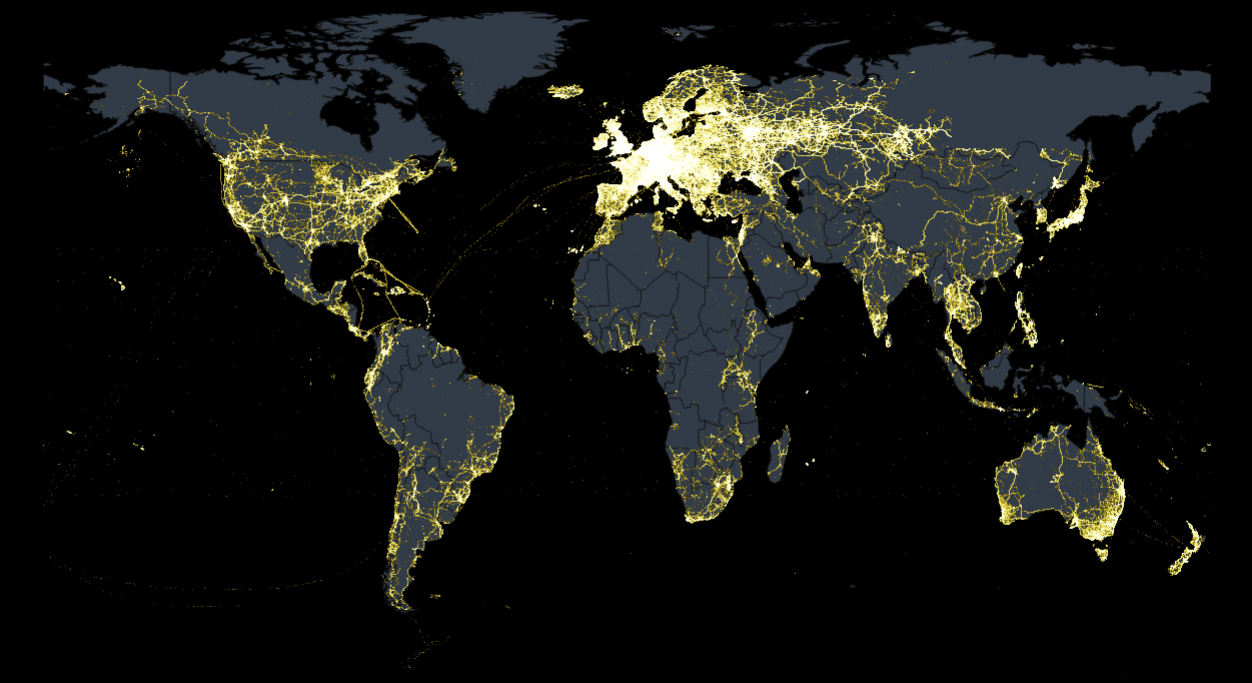
\includegraphics[width=0.9\textwidth]{country_GPS.png}
	\caption{Development in different parts of the world}\label{fig:cnt_GDP}
\end{figure}

This figure reflects the development of each area in the world.

\begin{figure}[H]
\centering
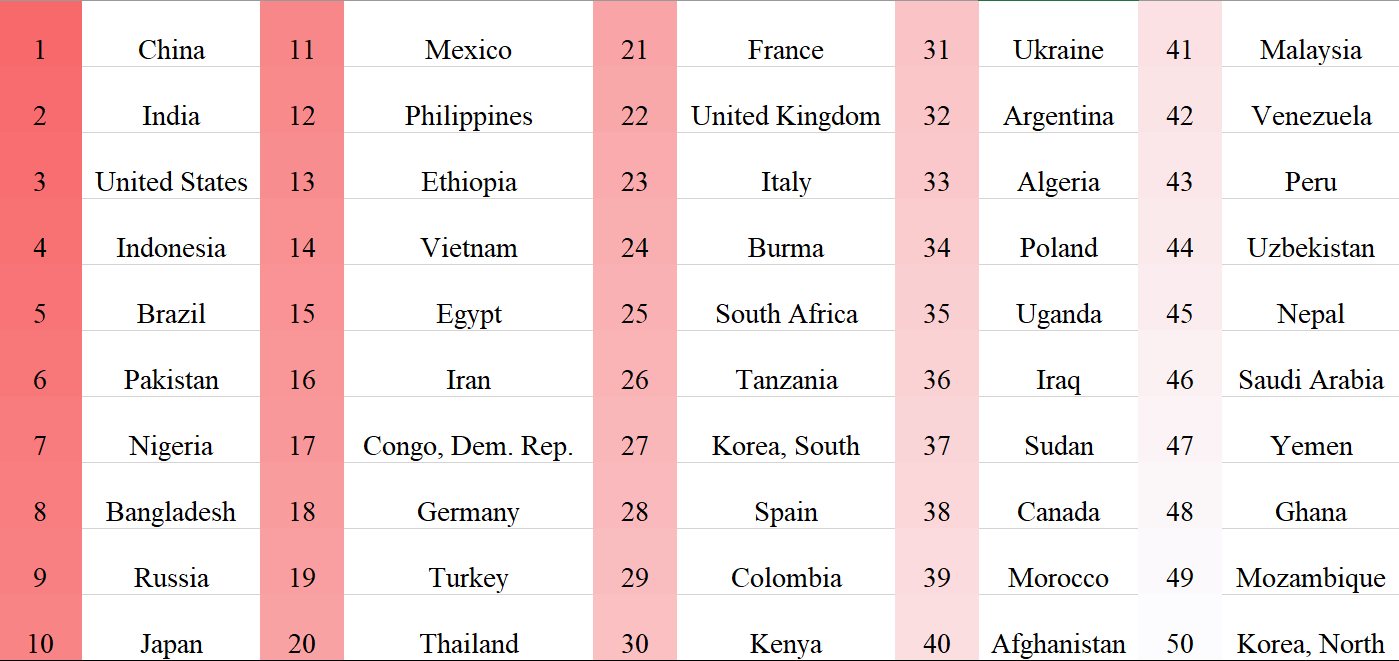
\includegraphics[width=0.9\textwidth]{countries.png}
\caption{50 candidate countries}\label{fig:cnt}
\end{figure}

Since China and USA had been selected as the office locations, our model is for the remaining 48 countries.

We use the topsis method to determine the office location, and use the entropy method, CRITIC method, and Standard deviation method to set the corresponding weights for each indicator. After the office location is initially determined, we use k-means clustering analysis to determine the office service area. After that, a series of indicators were used to re-score the service effect of different office locations and office areas, and comprehensively determine the best office locations and number. Here are the flow chart of our model:
\begin{figure}[H]
	\centering
	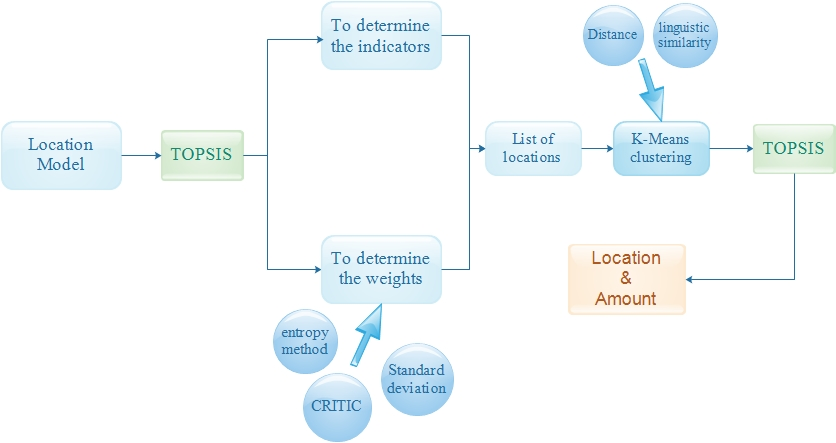
\includegraphics[width=0.8\textwidth]{process.jpg}
	\caption{flow chart of our model}\label{fig:flow_chart}
\end{figure}
\subsubsection{Weighted-Topsis}
The Topsis method was first proposed by C.L.Hwang and K.Yoon in 1981. The TOPSIS method is based on the closeness of a limited number of evaluation objects to the idealized target. It is a relatively good evaluation of the existing objects. The TOPSIS method is a sorting method that approximates the ideal solution. This method only requires that the utility functions be monotonically increasing (or decreasing). TOPSIS method is a commonly used effective method in multi-objective decision analysis, also known as the pros and cons solution distance method. The basic principle is to sort by detecting the distance between the evaluation object and the optimal solution and the worst solution. If the evaluation object is closest to the optimal solution and farthest from the worst solution, it is the best; otherwise it is not optimal. The value of each index of the optimal solution reached the optimal value of each evaluation index. The values ​​of each index of the worst solution reached the worst value of each evaluation index.

 In TOPSIS method, "ideal solution" and "negative ideal solution" are the two basic concepts of TOPSIS method. The so-called ideal solution is a conceived optimal solution (scheme), each attribute value of which reaches the best value of each alternative; the negative ideal solution is a conceived worst solution (scheme), it Each attribute value of is the worst value in each alternative. The rule for ordering the schemes is to compare the alternatives with the ideal solution and the negative ideal solution. If one of the schemes is closest to the ideal solution and at the same time is far away from the negative ideal solution, the scheme is the best solution among the alternatives.
 
 In the Weighted-Topsis method in our model, there are 2 types of the indicators:
 
 \begin{table}[H]
 	\begin{center}
 	\caption{2-types of the indicators in our model}
 	\begin{tabular}{|c|c|}
 		\hline
 		Benefit indicator & The goal is to maximize the indicator  \\ \hline
 		Cost indicator    & The goal is to miniimize the indicator \\ \hline
 	\end{tabular}
\end{center}
 \end{table}

According to the indicators given in the title and our considerations, we finally chose 6 indicators. They reflect a series of comprehensive factors such as market, cost, language, service range, etc., and can well consider whether an address is suitable as an office. Here are our indicators:

\begin{figure}[H]
	\centering
	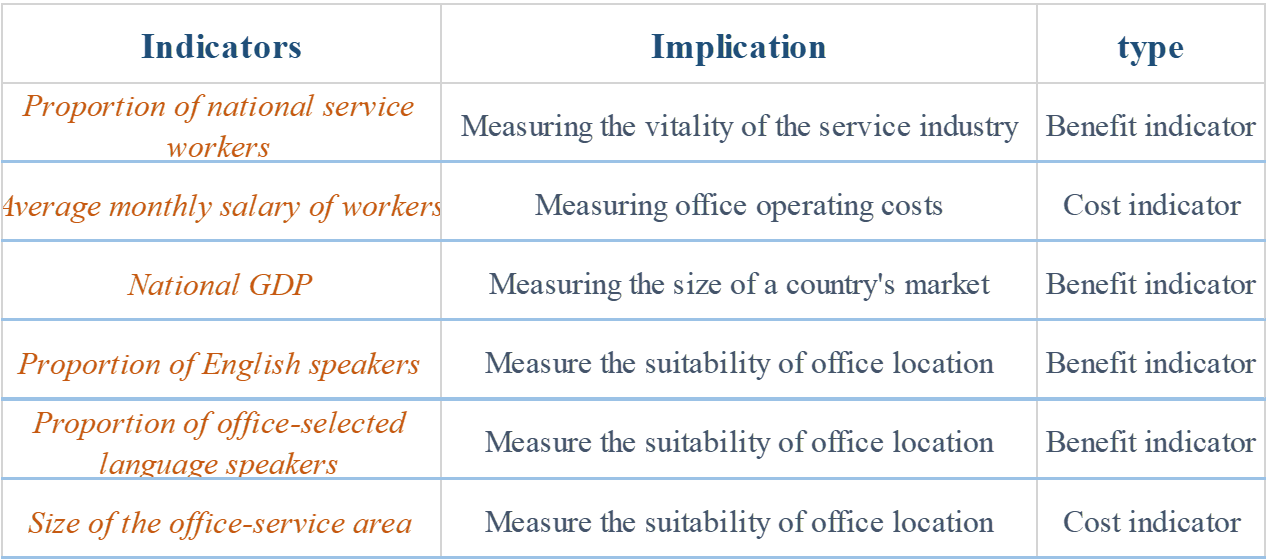
\includegraphics[width=1.0\textwidth]{indicators.png}
	\caption{indicators of our model}\label{fig:indicators}
\end{figure}

The Proportion of national service workers, Average monthly salary of workers, National GDP and Proportion of English speakers are used in our first layer of the topsis, and the Proportion of office-selected language speakers and Size of the office-service area are added in the second layer of the topsis after the area has been clustered by K-means method.

The following paragraphs describe the steps to use topsis on our model.

\begin{enumerate}[\bfseries 1.]
	\item \textbf{Unified indicator type.}
	
	Turn all indicators into benefit indicators. The second indicator and the last indicator of our model are the cost indicator, we need to turn them into benefit indicator by using:
	\begin{equation}
		\max  - x
	\end{equation}
	After this, we can get forward matrix X.
	
	\item \textbf{Standardized forward matrix}
	
	In order to eliminate the influence of different index dimensions, the matrix needs to be processed.
	
	Assume that there are n evaluation objects and m evaluation indexes that have been forwarded. The forward matrix formed is as follows:
	\begin{equation}
	X = \left[ {\begin{array}{*{20}{c}}
		{{x_{11}}}&{{x_{12}}}& \cdots &{{x_{1m}}}\\
		{{x_{21}}}&{{x_{22}}}& \cdots &{{x_{2m}}}\\
		\vdots & \vdots & \ddots & \vdots \\
		{{x_{n1}}}&{{x_{n2}}}& \cdots &{{x_{nm}}}
		\end{array}} \right]\
	\end{equation}
	The matrix to which it is normalized is called Y, and for each element ${y_{ij}}$ in Y:
	\begin{equation}
	{y_{ij}} = \frac{{{x_{ij}}}}{{\sqrt {\sum\limits_{i = 1}^n {{x_{ij}}^2} } }}
	\end{equation}
	
	\item \textbf{Calculate weighted matrix}
	
	Because the impact of each indicator is different, we need to assign a value to each indicator. The weighted matrix is called Z, and each element in Z:
	\begin{equation}
	{z_{ij}} = {w_i} \times {y_{ij}}
	\end{equation}
	We will discuss the method of empowerment later.
	
	\item \textbf{Calculate score and normalize}
	
	After the above steps, we get the weighted normalized matrix Z:
	\begin{equation}
	Z = \left[ {\begin{array}{*{20}{c}}
		{{z_{11}}}&{{z_{12}}}& \cdots &{{z_{1m}}}\\
		{{z_{21}}}&{{z_{22}}}& \cdots &{{z_{2m}}}\\
		\vdots & \vdots & \ddots & \vdots \\
		{{z_{n1}}}&{{z_{n2}}}& \cdots &{{z_{nm}}}
		\end{array}} \right]
	\end{equation}
	
	Define maximum value ${Z^ + }$ and minimum value ${Z^ -}$:
	\begin{equation}
	\begin{array}{l}
	{Z^ + } = \left( {{Z_1}^ + ,{Z_2}^ + , \cdots {Z_m}^ + } \right)\\
	= \left( {\max \left\{ {{z_{11}},{z_{21}}, \cdots ,{z_{n1}}} \right\},\max \left\{ {{z_{12}},{z_{22}}, \cdots ,{z_{n2}}} \right\}, \cdots ,\max \left\{ {{z_{1m}},{z_{2m}}, \cdots ,{z_{nm}}} \right\}} \right)\\
	\\
	{Z^ - } = \left( {{Z_1}^ - ,{Z_2}^ - , \cdots {Z_m}^ - } \right)\\
	= \left( {\min \left\{ {{z_{11}},{z_{21}}, \cdots ,{z_{n1}}} \right\},\min \left\{ {{z_{12}},{z_{22}}, \cdots ,{z_{n2}}} \right\}, \cdots ,\min \left\{ {{z_{1m}},{z_{2m}}, \cdots ,{z_{nm}}} \right\}} \right)
	\end{array}
	\end{equation}
	
	Define the distance between the i-th $\left( {i = 1,2, \cdots ,n} \right)$ evaluation object and the maximum value as ${D_i}^ + $:
	\begin{equation}
	{D_i}^ +  = \sqrt {\sum\limits_{j = 1}^m {{{\left( {{Z_j}^ +  - {z_{ij}}} \right)}^2}} }
	\end{equation}
	
	Define the distance between the i-th $\left( {i = 1,2, \cdots ,n} \right)$ evaluation object and the minimum value as ${D_i}^ - $:
	\begin{equation}
	{D_i}^ -  = \sqrt {\sum\limits_{j = 1}^m {{{\left( {{Z_j}^ -  - {z_{ij}}} \right)}^2}} }
	\end{equation}
	
	Then we can calculate the score of the i-th $\left( {i = 1,2, \cdots ,n} \right)$ evaluation object ${S_i}$:
	\begin{equation}
	{S_i} = \frac{{{D_i}^ - }}{{{D_i}^ -  + {D_i}^ + }}
	\end{equation}
\end{enumerate}

Next we explain how to weight indicators.

Entropy Method, Standard Deviation, CRITIC---The principle of these three methods is based on the degree of variation of the indicator. When the degree of variation of the indicator is smaller, the amount of information reflected is less and the corresponding weight is lower. 

Since the weights given in one way may have large deviations, we combine the three methods to give weights, and analyze the deviations to give the index weights in two ways, which give less deviation.

\begin{itemize}
	\item \textbf{Entropy Method}
	
	Let m indicators of n evaluation objects have been normalized as $y_{ij} \left( {i = 1,2, \cdots ,n;j = 1,2, \cdots m} \right)$. The information entropy of the j-th index is:
	\begin{equation}
	{E_j} =  - \frac{{\sum\limits_{i = 1}^n {{p_{ij}}\ln {p_{ij}}} }}{{\ln n}}\left( {i = 1,2, \cdots ,n;j = 1,2, \cdots ,m} \right)
	\end{equation}
	and ${p_{ij}} = \frac{{{y_{ij}}}}{{\sum\limits_{i = 1}^n {{y_{ij}}} }}$.
	When E is smaller, the difference between the data is larger, so the larger the information provided, the greater the weight of the indicator, and vice versa.
	
	Then we can get the calculation formula of objective weight:
	\begin{equation}
	{w_j} = \frac{{1 - {E_j}}}{{m - \sum\limits_{j = 1}^m {{E_j}} }}(j = 1,2, \cdots m)
	\end{equation}
	
	\item \textbf{Standard Deviation}
	
	Unlike the calculation of information entropy, in the standard deviation method, we use the method of calculating standard deviation to measure the amount of information provided by an indicator. When the standard deviation is large, we think that it provides more information. When the standard deviation is small, we think it provides less information.
	
	The calculation as following:
	\begin{equation}
	{w_j} = \frac{{{\sigma _j}}}{{\sum\limits_{j = 1}^m {{\sigma _j}} }}(j = 1,2, \cdots ,m)
	\end{equation}
	where $\sigma _j$ represents the standard deviation.
	
	\item \textbf{CRITIC}
	
	The CRITIC method weights indicators based on two basic concepts: The first is contrast. When the standard deviation is larger, the weight is relatively larger. The second is to evaluate the conflict between indicators. Here we introduce the correlation coefficient r between indicators. When there is a strong positive correlation between indicators, it means that the conflict between the two indicators is low, and the information reflected by the two indicators is relatively similar. When there is a strong negative correlation between the two indicators, it means that the conflict between the two indicators is large, and the information reflected by the two indicators is quite different.
	
	The calculation as following:
	
	The amount of information contained in the j-th indicator is:
	\begin{equation}
	{c_j} = {\sigma _j}\sum\limits_{i = 1}^m {(1 - {r_{ij}})(j = 1,2, \cdots ,m)} 
	\end{equation}
	where ${r_{ij}}$ represents the correlation coefficient between the i-th indicator and j-th indicator.
	
	Then we get the j-th indicator's weight:
	\begin{equation}
	{w_j} = \frac{{{c_j}}}{{\sum\limits_{i = 1}^m {{c_i}} }}(j = 1,2, \cdots ,m)
	\end{equation}
\end{itemize}

\subsubsection{Weighted K-Means Clustering}
After the first usage of the Weighted-Topsis, we get the score of each country among the 50-countries' list. Considering that each office needs to serve an area, we introduce Weighted K-Means Clustering to determine the area that one office needs to serve.

K-means is a certain distance from the data point to the prototype as the objective function of the optimization, and the method of calculating the extreme value of the function is used to obtain the adjustment rule of the iterative operation. The K-means algorithm uses Euclidean distance as a similarity measure. It seeks the optimal classification corresponding to a certain initial clustering center vector MC, so that the evaluation index D is minimized. The algorithm uses the sum of squared error function as the clustering criterion function. Eventually, the obtained clusters satisfy the similarity of objects in the same cluster, and the cluster center and the objects assigned to them represent a cluster.

\begin{figure}[H]
	\centering
	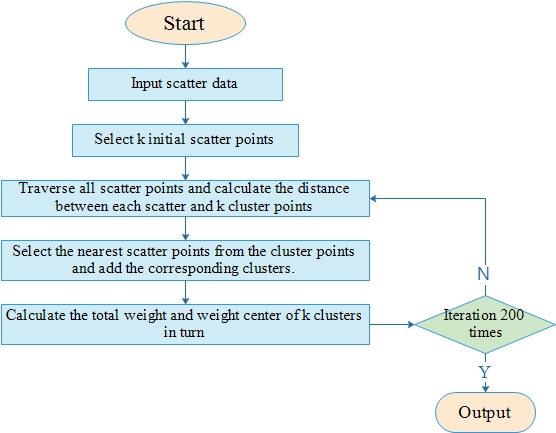
\includegraphics[width=0.7\textwidth]{K-means.jpg}
	\caption{flow chart of K-Means Clustering}\label{fig:K-means}
\end{figure}

The core formula of the K-means algorithm:
\begin{equation}
D\left( {\left\{ {{\pi _c}} \right\}_{c = 1}^k} \right) = \sum\limits_{c = 1}^k {\sum\limits_{a,e{x_c}} {{{\left\| {{a_i} - {m_c}} \right\|}^2}} } ,{\rm{ where }}{m_c} = \frac{{\sum\limits_{a, \in {\pi _c}} {{a_i}} }}{{\left| {{\pi _c}} \right|}}
\end{equation}
${a_{ij}},\left( {i = 1,2,...,n;j = 1,2,...,m} \right)$ refers to all of the elements. And here m=2, means the longitude and latitude, which is the location of the center point(At first is the office selected.). ${\pi _c}$ means the cluster group and the total number is k. ${m_c}$ is the cluster center of the element ${a_i}$ in group ${\pi _c}$. After continuous iteration we can get the final clustering result.

Through the k-means algorithm, we can obtain a good regionalization scheme from the initial center point and continuous iteration. Here is an example:

\begin{figure}[H]
	\begin{minipage}[t]{0.3\linewidth}
		\centering
		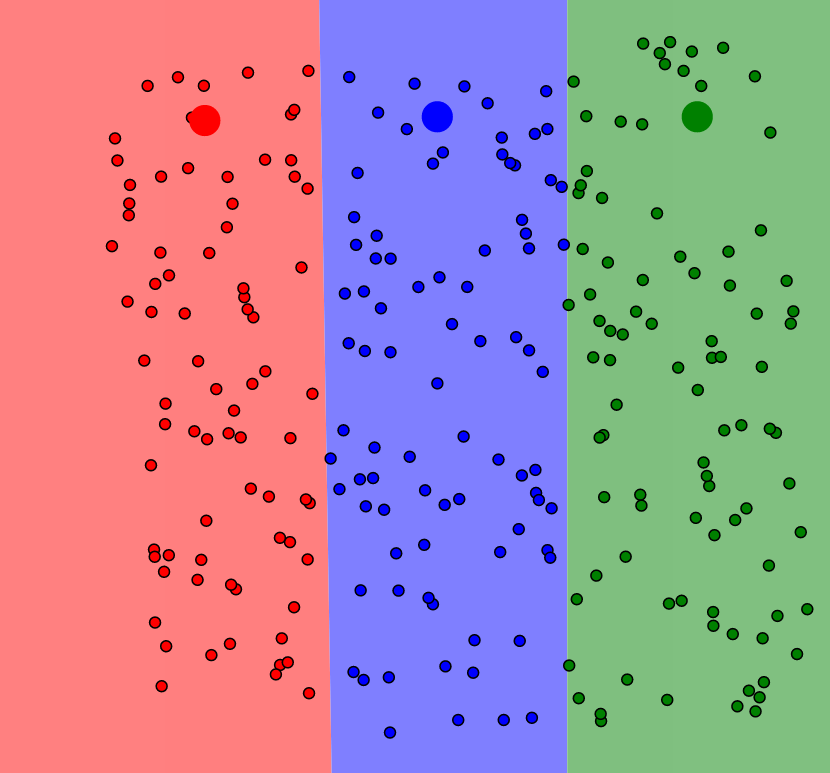
\includegraphics[height=4cm,width=4cm]{k-means_1.png}
		\caption{Init}
	\end{minipage}%
	\hfill
	\begin{minipage}[t]{0.3\linewidth}
		\centering
		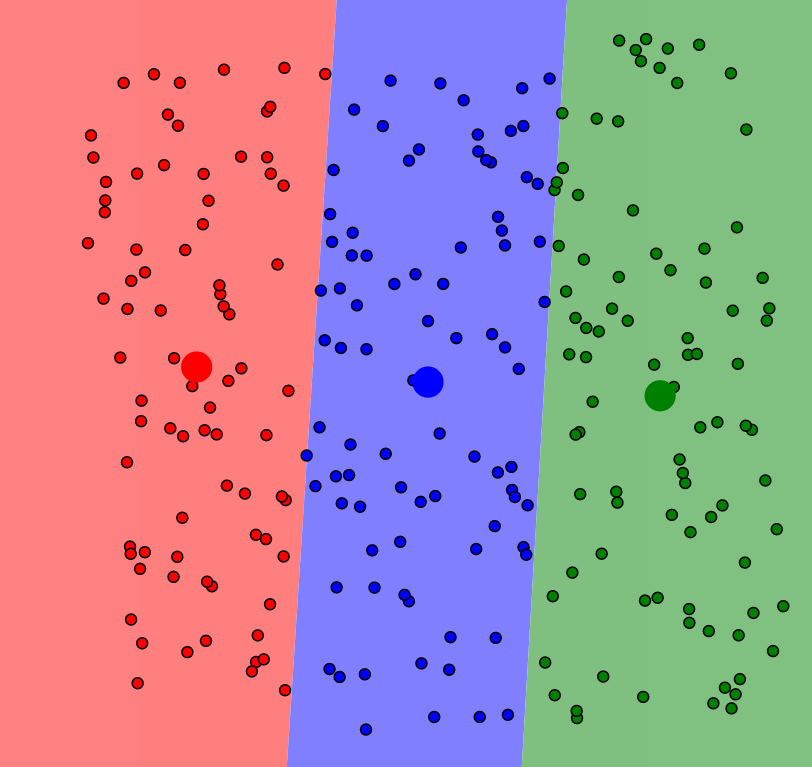
\includegraphics[height=4cm,width=4cm]{k-means_2.png}
		\caption{After 10 iterations}
	\end{minipage}
	\hfill
	\begin{minipage}[t]{0.3\linewidth}
		\centering
		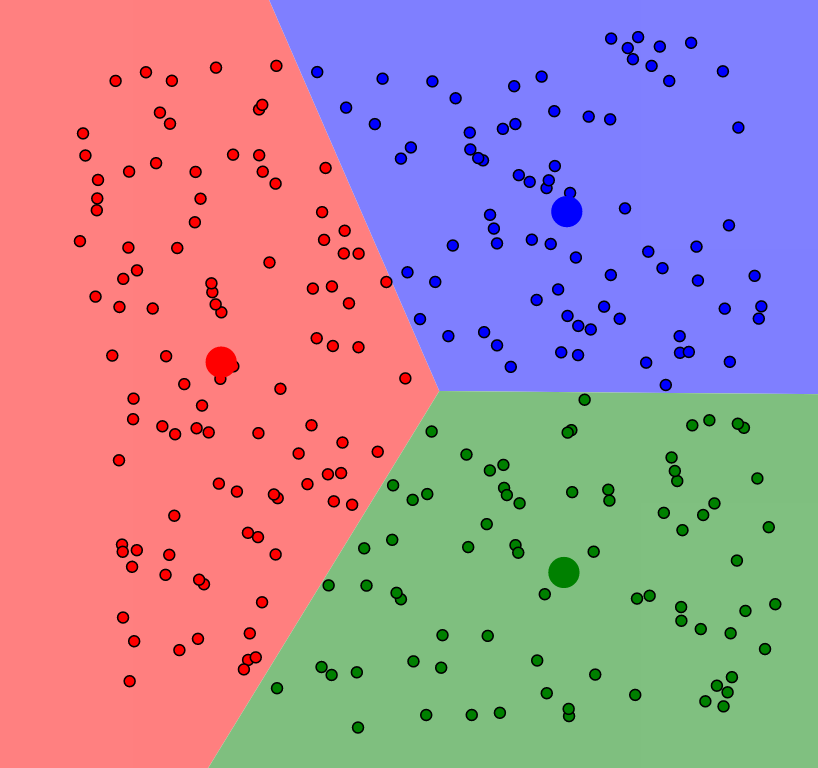
\includegraphics[height=4cm,width=4cm]{k-means_3.png}
		\caption{After 50 iterations}
	\end{minipage}
\end{figure}

From the example we can see the cluster center in the final cluster compared to the original has a large offset. This means the K-Means clustering is not enough to solve our location model. Since the K-means clustering model uses a 1: 1 ratio for the distance comparison of each scattered point set, but for us, we need to consider not only the straight line distance between the capital and the cluster center, but also to the language similarity and other factors. If we use distance as the sole criterion, then it is better to define the service area according to the radiation range centered on the country. Because then the office location we originally selected will not change. However, Based on our considerations, the reason we apply the k-means algorithm is as follows:
\begin{itemize}
	\item Introduce language similarity as weights to help us flexibly divide regions.
	\item Judging the correctness and appropriateness of the initial choice by observing the change in the center point. If the center point has a large deviation, it means that the initially selected point is not suitable as an office. Then we can consider changing the location or country for better results.
\end{itemize}

Based on the above ideas, we apply the 了Weighted K-Means Clustering to solve our model.

The core formula of the Weighted K-means Clustering:
\begin{equation}
D\left( {\left\{ {{\pi _c}} \right\}_{c = 1}^k} \right) = \sum\limits_{c = 1}^k {\sum\limits_{{a_i} \in {\pi _c}} {w_i^y} } {\left\| {{a_i} - {m_c}} \right\|^2},\quad {\rm{ where }}{m_c} = \frac{{\sum\limits_{a,e{\pi _c}} {w_i^y} {a_i}}}{{\sum\limits_{{a_i} \in {\pi _c}} {w_i^y} }}
\end{equation}
The calculation method of this formula is very similar to the k-means algorithm, except that for different sample points, a corresponding weight wi and a weight attenuation coefficient y are multiplied. Here we set the y=1.


\subsubsection{Solution and Analysis of Location Model}

Via the data we collected, we quantified six indicators and normalized these indicators. Running the Entropy Method, Standard Deviation, CRITIC respectively. We get three different weight vectors as following:

\begin{center}
Entropy Method:
${\left[ {\begin{array}{*{20}{c}}
		{\begin{array}{*{20}{c}}
			{\begin{array}{*{20}{c}}
				{0.22}\\
				{0.25}
				\end{array}}\\
			{0.31}
			\end{array}}\\
		{0.22}
		\end{array}} \right]^{ - 1}}$
	
Standard Deviation:
${\left[ {\begin{array}{*{20}{c}}
		{\begin{array}{*{20}{c}}
			{\begin{array}{*{20}{c}}
				{0.14}\\
				{0.39}
				\end{array}}\\
			{0.32}
			\end{array}}\\
		{0.15}
		\end{array}} \right]^{ - 1}}$
		
CRITIC:
${\left[ {\begin{array}{*{20}{c}}
		{\begin{array}{*{20}{c}}
			{\begin{array}{*{20}{c}}
				{0.30}\\
				{0.15}
				\end{array}}\\
			{0.35}
			\end{array}}\\
		{0.20}
		\end{array}} \right]^{ - 1}}$
\end{center}

We calculated the rankings obtained by topsis under the three kinds of weights, and finally selected 12 countries. Considering that a country's capital often best reflects its economic level. At the beginning, we assumed that the national capital was the office location. As for the choice of language: we assume the most spoken language in the region other than English as the language the office selected to use.

\begin{figure}[H]
	\centering
	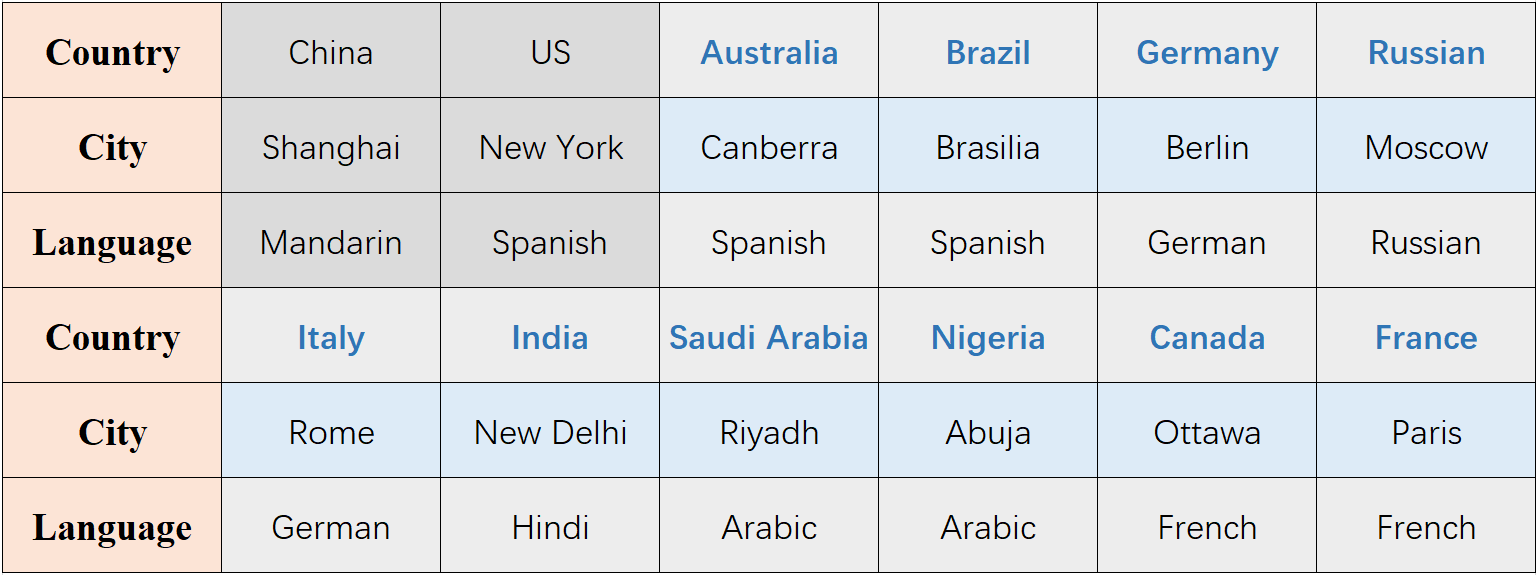
\includegraphics[width=1\textwidth]{first_select.png}
	\caption{Selected location by topsis}\label{fig:first_select}
\end{figure}
Because China and the United States have been selected as office locations, we just need to consider the other 10 regions. The selection of China and the United States also proved the correctness of the first site selection in our model.

After the Weighted-Topsis, we tried the choices of 6 different countries among lists and brought them into the k-means cluster with distance and language consistency and country relations as weights to divide the service area for the selected office. 

Later, the regional division was completed, we brought the next two indicators to recalculate the score of topsis, and selected the highest 6 locations in different divisions by clustering. 

After multiple assignments we found that when we use Germany, Brazil, Australia, Nigeria, Russian and India as the locations of the office, we can receive the highest benifit and lowest cost. The deviation of the cluster center is also little, which means the capital is suitable for the location. And we find that when we use different combination, the 6 highest average scores are also these countries. Here is the score in average:
\begin{figure}[H]
	\centering
	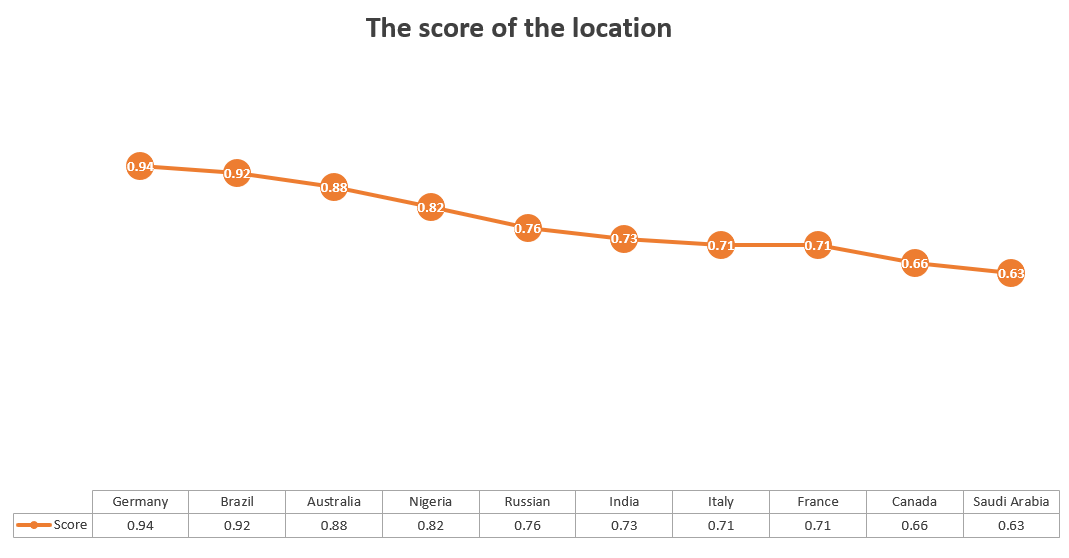
\includegraphics[width=0.9\textwidth]{Location_Score.png}
	\caption{Score of the location}\label{fig:location}
\end{figure}

For determing the best amount of the offices, we just need to make minor changes to our model, since the amount does not affect the score. We can know from the supervisor's analysis that when we cut down the amount of the offices, the office construction costs and operating costs will decrease, but revenue and service intensity will increase. Our indicators take these points into account, so we can continue to use our model rather than change the indicators. Finally, by running our models, we find that building 6 offices in these countries is still the most suitable. At this point, our model is solved, and we give the distribution of our offices in World Map:
\begin{figure}[H]
	\centering
	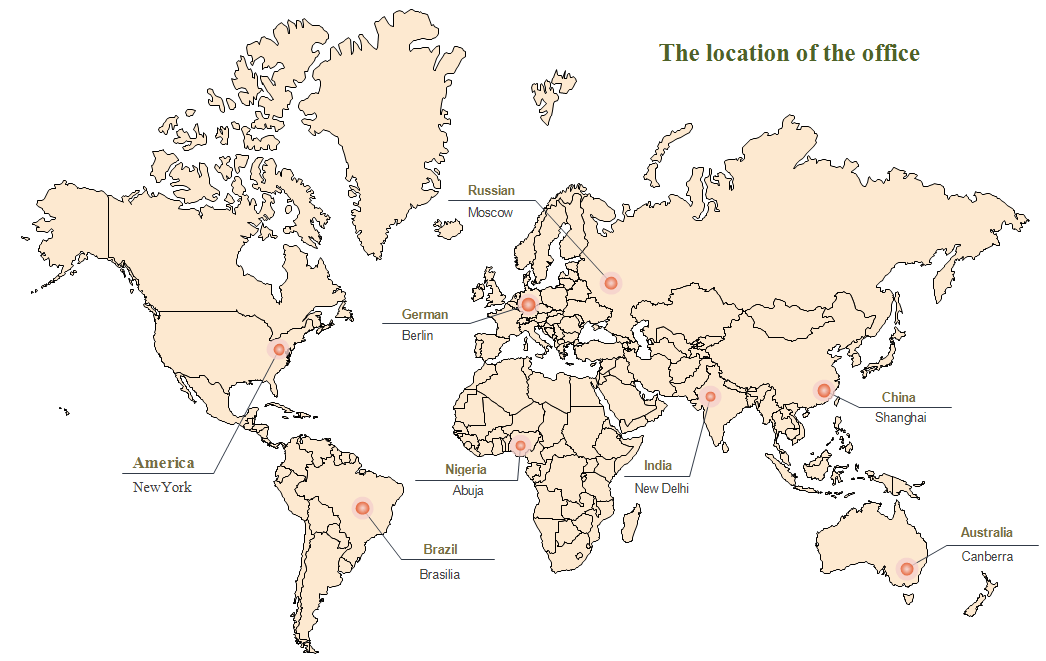
\includegraphics[width=1\textwidth]{location.png}
	\caption{location of the offices}\label{fig:offices}
\end{figure}

\subsubsection{Sensitivity Analysis}

For problem 2, because our model considers more comprehensive factors, it can be consistent in the short and long term. Here we give a sensitivity analysis on time.

Based on our initial scores, the values and scores of the six selected countries are shown below.

\begin{figure}[H]
	\centering
	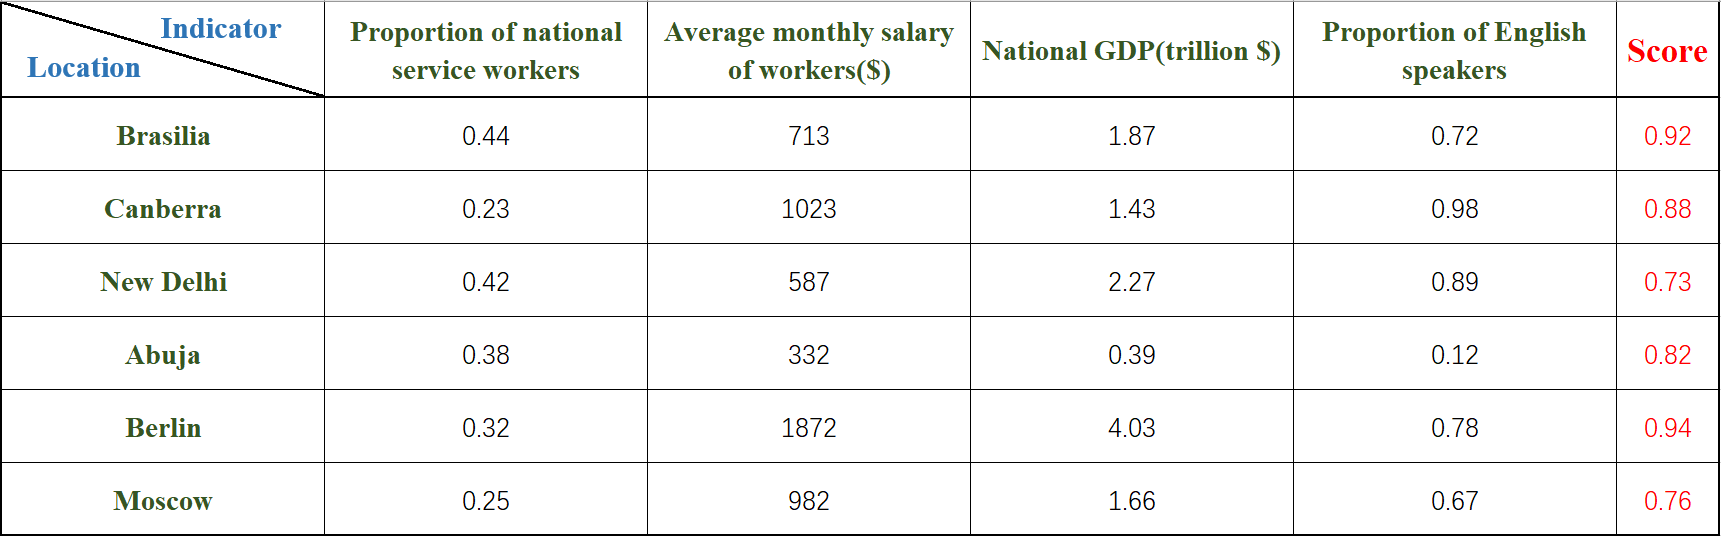
\includegraphics[width=1\textwidth]{Sensitivity.png}
	\caption{Short-term Score}\label{fig:sensitivity}
\end{figure}

According to our analysis, over time, when a country begins to develop, its number of English speakers will increase, and GDP will increase. These are all contributing factors, but the decline in service practitioners and the increase in per capita wages will be restrained. Effect, according to our prediction, this promotion and inhibition effect will maintain the stability of the score. This effect is predictable, because in the initial country selection, we not only considered the current development level of this country, but also considered the potential development potential of developing countries.

\begin{figure}[H]
	\centering
	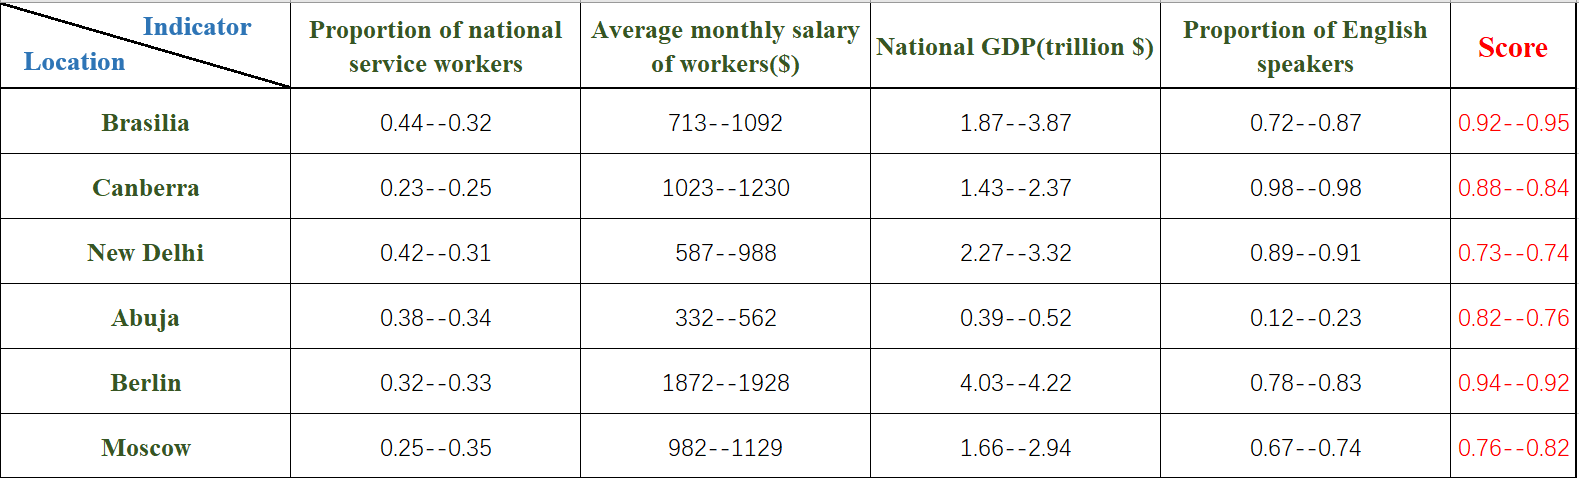
\includegraphics[width=1\textwidth]{Sensitivity_1.png}
	\caption{Long-term Score}\label{fig:sensitivity_1}
\end{figure}

As can be seen from the above figure, in the long-term development process, our best choice is still these six countries, and the scores have not changed much.













\section{Strengths and Weaknesses}
\subsection{Strengths}
\begin{itemize}
    \item First one...
    \item Second one ...
\end{itemize}

\subsection{Weaknesses}
\begin{itemize}
    \item Only one ...
 \end{itemize}


% 以下为信件/备忘录部分,不需要可自行去掉
% 如有需要可将整个 letter 环境移动到文章开头或中间
% 请在后一个花括号内填写信件(Letter)或备忘录(Memorandum)标题
\begin{center}
	\textbf{Memo}
\end{center}
\begin{letter}{}
\begin{flushleft}  % 左对齐环境,无首行缩进
\textbf{To:} Heishan Yan\\
\textbf{From:} Team XXXXXXX\\
\textbf{Date:} October 1st, 2019\\
\textbf{Subject:} A better choice than MS Word: \LaTeX
\end{flushleft}

In the memo, we want to introduce you an alternate typesetting program to the prevailing MS Word: \textbf{\LaTeX}. In fact, the history of \LaTeX\ is even longer than that of MS Word. In 1970s, the famous computer scientist Donald Knuth first came out with a typesetting program, which named \TeX\ \ldots

Firstly, \ldots

Secondly, \ldots

Lastly, \ldots

According to all those mentioned above, it is really worth to have a try on \LaTeX! 
\end{letter}


% 参考文献,此处以 MLA 引用格式为例
\begin{thebibliography}{99}
\bibitem{1} Einstein, A., Podolsky, B., \& Rosen, N. (1935). Can quantum-mechanical description of physical reality be considered complete?. \emph{Physical review}, 47(10), 777.
\bibitem{2} \emph{A simple, easy \LaTeX\ template for MCM/ICM: EasyMCM}. (2018). Retrieved December 1, 2019, from\url{https://www.cnblogs.com/xjtu-blacksmith/p/easymcm.html}
\end{thebibliography}


% 以下为附录内容
% 如您的论文中不需要附录,请自行删除
\begin{subappendices}  % 附录环境

\section{Appendix A: Further on \LaTeX}
To clarify the importance of using \LaTeX\ in MCM or ICM, several points need to be covered, which are \ldots

To be more specific, \ldots

All in all, \ldots

Anyway, nobody \textbf{really} needs such appendix \ldots

\end{subappendices}

\end{document}  % 结束